% Elsevier CAS single-column template (els-cas-templates, cas-sc).
\documentclass[a4paper,fleqn]{cas-sc}

% Compile this Chinese manuscript with XeLaTeX.
\usepackage[UTF8]{ctex}
\usepackage[authoryear]{natbib}
\usepackage{bm}
\usepackage{tikz}
\usetikzlibrary{arrows.meta,positioning,shapes.geometric,fit}
\usepackage{enumitem}
\usepackage{threeparttable}
\hypersetup{colorlinks=true,linkcolor=black,citecolor=black,urlcolor=blue}
\ExplSyntaxOn
\bool_gset_true:N \g_stm_nologo_bool
\ExplSyntaxOff

% Shared notation for AgriOcc.
\newcommand{\R}{\mathbb{R}}
\newcommand{\I}{\mathcal{I}}
\newcommand{\B}{\mathcal{B}}
\newcommand{\V}{\mathcal{V}}
\newcommand{\Y}{\mathcal{Y}}
\newcommand{\softmax}{\operatorname{softmax}}
\newcommand{\CE}{\operatorname{CE}}
\newcommand{\KL}{\operatorname{KL}}
\newcommand{\IoU}{\operatorname{IoU}}
\newcommand{\mIoU}{\operatorname{mIoU}}
\newcommand{\argmax}{\operatornamewithlimits{arg\,max}}

\begin{document}
\let\WriteBookmarks\relax
\def\floatpagepagefraction{1}
\def\textpagefraction{.001}

\shorttitle{AgriOcc}
\shortauthors{He, Jin, Liu and Qu}

\title[mode=title]{AgriOcc：面向农业机器人的几何感知高效三维语义占用预测模型}

\author[1]{Lei He}
\author[1]{Jing Jin}[orcid=0000-0001-7753-7656]
\cormark[1]
\ead{jinjinghit@hit.edu.cn}
\author[2]{Yi Liu}
\affiliation[1]{
  organization={School of Astronautics, Harbin Institute of Technology},
  city={Harbin},
  postcode={150001},
  country={China}
}
\affiliation[2]{
  organization={Zhengzhou Advanced Research Institute of Harbin Institute of Technology},
  city={ZhengZhou},
  postcode={450000},
  country={China}
}

\begin{abstract}
农业机器人的视觉导航通常依赖二维图像内的作物行检测、可通行区域分割及相应后处理技术。
现有二维感知链路易在几何拟合与坐标转换中累积误差，也难以为不同作物和机器人平台提供统一的参数和接口。
本文提出 AgriOcc：一种从三路前视 RGB 图像端到端预测机器人前方三维语义占用的框架，为田间作业、避障和导航提供统一的体素化环境表征。
AgriOcc 的核心由 GeoVis-BEV 编码器和农业结构自适应混合专家三维占用解码器（Agri-AMoE）构成。
GeoVis-BEV 编码器在多相机 BEV 表征学习中协同引入几何可见锚点可变形注意力（GVAD）和近远场查询布局：前者从可靠可见区域汇聚长程上下文，并保留局部可变形采样；后者将编码预算集中于近场精细结构，同时对远场查询进行规则稀疏化与特征恢复。
Agri-AMoE 将 BEV 表征提升为三维特征体，先以通道注意力增强特征，再利用空间显著性和梯度能量在局部平面、垂直结构和大范围上下文专家之间自适应路由。
针对农业语义占用数据稀缺且采集成本高的问题，本文构建了农业多视角仿真数据集 AgriOcc-Dataset。
在该数据集上，AgriOcc 取得 56.99\% mIoU，优于所对比的多相机语义占用方法；
在真实越野数据集 ORAD-3D 上，以本文数据预训练可将目标域适配时间由 54.1 分钟缩短至 18.5 分钟，并在取得性能的明显提升。
实验表明，AgriOcc 具备农业场景理解与真实环境迁移能力，为农业移动机器人的三维视觉导航提供了兼顾精度与训练开销的新路径。
\end{abstract}
\begin{keywords}
农业机器人 \sep 三维语义占用预测 \sep 鸟瞰表征 \sep 仿真到真实迁移 \sep 多相机视觉
\end{keywords}

\maketitle

% The complete manuscript is kept in this file.  The historical files in
% sections/ are retained only as backups and are not part of the build.

\section{引言}\label{sec:intro}

农业机器人在田间执行巡检、植保、收获运输和自主导航时，需要同时理解作物、垄沟、土壤、
可通行区域与突发障碍物的空间关系。现有视觉导航系统通常采用模块化流程：
先通过作物行识别、道路或可通行区域分割得到二维结果，再经几何拟合、
坐标变换和规则后处理生成导航约束\citep{nkwochaComprehensiveReviewSensing2025,baiVisionbasedNavigationGuidance2023}。
该流程存在两个限制：
其一，二维感知、几何恢复和控制坐标变换彼此分离，前级预测误差会逐级传播；
其二，作物品种、田块结构或机器人平台变化后，感知模型和后处理规则往往需要重新设定。
对于具有密集植株、连续垄行和复杂遮挡的农田，仅以二维像素级结果作为导航接口也难以表达高度、
遮挡后空间与株间间隙。

三维语义占用预测以机器人自身坐标系中的规则体素网格统一表示环境，
每个体素给出占据状态或语义类别。它能够将自由空间、地面、作物和障碍物以统一接口
提供给后续通行性分析、碰撞检查和视觉导航。
自动驾驶研究已证明，Lift--Splat--Shoot 等显式提升方法\citep{philion2020lift,huang2021bevdet,li2022bevdepth}，
以及 DETR3D、PETR 和 BEVFormer 等查询式方法\citep{wang2022detr3d,li2022petr,li2022bevformer}，
都可从多相机图像学习几何一致的鸟瞰表征；该表征还能扩展至稠密占用\citep{wei2023surroundocc,wang2023openoccupancy}、
时序场景预测和规划\citep{zheng2024occworld,mei2025irwm}。
这些方法常设定六路环视相机、面向全向道路交通场景，并使用较大时空范围与模型规模。
而农业机器人则通常配备低算力平台，多在相对静态、前向作业的田间环境中运行。

因此本文聚焦农业机器人最常见的前向作业视野：输入正前、左前和右前三路相机，
预测前方 $20\,$m 的三维语义占用。然而，农业领域因受到作物生长阶段、地块变化、传感器配置等限制，
难以形成如 nuScenes 这类规模化的自动驾驶数据集。现有研究往往也只针对一种作物，难以进行跨地域、跨作物种类的泛化性研究。
为建立全面、多样、可控的训练与评测环境，
本文首先基于 Unreal Engine 5 构建了 AgriOcc-Dataset：包含 298 个完整序列、38,862 帧多视角样本，
涵盖 10 种作物、3 个生长阶段、5 个时段及两类天气条件的农业语义占用数据。

现有语义占用方法在农业前向视野中仍面临三项关键挑战。
第一，不同 BEV 单元被三路相机直接观测的程度不同；仅依赖局部采样时，
弱可见区域难以获得可靠区域的结构化语义上下文。第二，
近场与远场的物理采样密度和语义细节存在显著差异，
维持全场稠密查询会将大量计算耗费在低细节远场。第三，作物边界、
植株高度变化与小尺度障碍具有强烈的三维局部结构，
将每个 BEV token 独立映射为高度 logits 的统一 MLP 容易平滑这些高梯度体素。
为此，本文提出 AgriOcc，如图\ref{fig:overview}所示。
整体框架由三相机图像编码器、GeoVis-BEV 编码器和 Agri-AMoE 三维占用解码器构成。
图像编码器先从三路图像提取多尺度特征，再通过相机投影将其聚合到机器人前方的 BEV 查询中。
GeoVis-BEV 编码器面向农业前向视野组织 BEV 表征学习：
其中，GVAD 将局部可变形图像采样与可见性加权的全局锚点上下文协同建模，
使弱观测单元能够从可靠可见区域获得结构化补全；
近远场查询布局则保持近场稠密计算，并对远场采用规则稀疏采样与特征恢复，
从而匹配不同距离区域的感知需求与计算预算。
最后，Agri-AMoE 将编码后的 BEV token 提升为三维特征体，先通过通道注意力增强，
再依据空间显著性、梯度能量以及平面、垂直和大范围上下文的结构差异自适应路由专家，端到端输出前方空间的六类语义体素。

我们的主要贡献如下：
\begin{enumerate}[leftmargin=1.8em]
  \item 构建面向农业机器人三维语义占用的仿真数据集 AgriOcc-Dataset：包含 298 个序列、38.8k 个样本，
        在机器人自身坐标系下统一提供六类前方环境体素标注，并给出可参数化的数据采集与自动标注流程；
  \item 提出 AgriOcc，据我们所知（截至 2026 年 9 月）首个面向农业移动机器人前向作业视野的三维语义占用预测模型。
        它通过端到端学习将三路前视 RGB 图像映射为前方空间的稠密语义体素，提供统一的农业环境三维表征；
  \item 提出 GeoVis-BEV 编码器，将几何可见锚点可变形注意力（GVAD）和近远场查询布局纳入统一的 BEV 表征学习过程：
        前者以可见锚点上下文补全弱观测区域，后者以近密远疏的查询分配匹配农业前向视野的距离差异；
  \item 提出 Agri-AMoE 占用解码器，将 BEV 表征提升为三维特征体，并以梯度能量自适应路由局部平面、垂直结构和大范围上下文专家；
\end{enumerate}

\section{相关工作}\label{sec:related}

\paragraph{多相机 BEV 感知}
鸟瞰（bird's-eye-view, BEV）表征将多相机图像中的视觉证据映射到机器人或车辆坐标系的俯视平面，使不同视角的观测能够在统一空间网格中进行融合、推理和规划。
以 BEV 为中间表征的视觉感知方法通过预定义空间查询把多相机图像特征对齐到该统一坐标系。
显式提升范式将图像特征沿深度分布投影至 BEV，代表性工作包括 Lift--Splat--Shoot、BEVDet、
BEVDepth 和 BEVStereo\citep{philion2020lift,huang2021bevdet,li2022bevdepth,li2022bevstereo}；
MatrixVT 则进一步讨论了高效的多相机到 BEV 变换\citep{zhou2022matrixvt}。
查询式方法则利用三维参考点、位置嵌入或跨视图变换直接读取相机特征\citep{wang2022detr3d,li2022petr,liu2023petrv2,li2023fbbev}，
并可在共享 BEV 中融合多模态信息\citep{liu2023bevfusion}。
BEVFormer 进一步以空间交叉注意力和时序自注意力建立 BEV 查询之间的几何关联\citep{li2022bevformer}。
这些方法为统一坐标系下的视觉感知奠定基础。

\paragraph{三维占用预测与高效表征}
视觉三维占用将自由空间和语义实体编码为稠密或压缩的体素场。MonoScene、TPVFormer 和 VoxFormer 分别从单目特征提升、
三平面表征和可见稀疏体素出发完成场景补全\citep{cao2022monoscene,huang2023tpvformer,li2023voxformer}；
SurroundOcc 与 OpenOccupancy 推动了多相机稠密占用预测和环视基准的发展\citep{wei2023surroundocc,wang2023openoccupancy}。
由于三维体素的计算代价随空间分辨率快速增长，后续工作从局部--全局结构、
紧凑或由粗到细的查询、稀疏交互，以及高效解码和渲染监督等方向降低开销\citep{zhang2023occformer,ma2024cotr,wang2024panoocc,liu2024sparseocc,tang2024sparseocc,yu2023flashocc,pan2024renderocc}。
占用表征也进一步扩展为时序世界模型：BEVDet4D、OccWorld、IR-WM 与 ForecastOcc 分别
利用跨帧 BEV、离散场景 token 或历史图像观测预测动态环境和未来状态\citep{huang2022bevdet4d,zheng2024occworld,mei2025irwm,mohan2026forecastocc}。
这些研究验证了占用作为统一空间接口的价值，但其普遍面向全向交通环境，
依赖更广的相机覆盖或历史运动信息。

\paragraph{农业与越野三维感知数据}
城市三维感知的常用数据集包括 KITTI\citep{geiger2012kitti}、SemanticKITTI\citep{behley2019semantickitti} 和 nuScenes\citep{caesar2020nuscenes}，
但它们的传感器布置、类别构成和道路结构与农田不同。
农业场景中的公开数据多面向作物行检测、二维语义分割、实例分割或特定作业目标，难以同时提供多相机标定和稠密三维语义体素；
越野方向的 RELLIS-3D\citep{jiang2020rellis} 也主要服务于多模态分割与建图。
虚拟驾驶平台 CARLA\citep{dosovitskiy2017carla} 及领域随机化\citep{tobin2017domainrandomization,peng2018sim2real}、
语义一致域适应\citep{hoffman2018cycada} 说明仿真环境可以极大地缓解真实世界数据采集成本高、周期长的难题，
这一点在农业场景中尤为突出。
在真实越野方向，ORAD-3D 提供涵盖农田、林地、草地和道路等场景的三维占用
基准\citep{chen2025orad3d}，为本文提供了真实场景下的验证途径。
需要说明的是，现有农业与越野三维感知工作多基于激光雷达或单目相机，
其传感器配置与任务定义均不同于本文的多路前视相机稠密语义占用预测，
因此未纳入本文的实验对比协议。据我们所知，目前面向农业机器人前向作业视野、
以多路前视相机直接输出机器人坐标系稠密三维语义占用的公开数据集与模型仍属空白，
本文的 AgriOcc-Dataset 与 AgriOcc 正是针对这一空缺提出的。

\section{方法}\label{sec:method}

\subsection{任务定义}\label{sec:task}
本文聚焦农业机器人最常见的前向作业视野：输入正前、左前和右前三路相机，预测前方 $20\,$m 的三维语义占用。
给定时刻 $t$ 的三路同步图像 $\I_t=\{I_t^{\mathrm{FL}},I_t^{\mathrm{F}},I_t^{\mathrm{FR}}\}$、
相机内外参和机器人坐标系，目标是在前向空间
\begin{equation}
\B=[0,20]\times[-10,10]\times[-2,3]~\mathrm{m}
\end{equation}
中预测语义占用。体素分辨率为 $0.2~\mathrm{m}$，因此输出网格为 $100\times100\times25$。
每个有效体素 $v\in\V$ 的标签 $y_v\in\{0,\ldots,5\}$ 分别表示自由空间、
作物、土壤地面、可通行区域（drivable）、其他植被与其他障碍物六类。

\subsection{仿真数据采集系统与AgriOcc-Dataset}\label{sec:dataset_construction}
\subsubsection{农田仿真数据采集系统}\label{sec:synthetic}
为缓和农业场景作物种类繁多、数据采集时间跨度大等问题带来的农机数据采集困难，
本文首先基于 Unreal Engine 5 构建可参数化农场仿真环境，其流程如图\ref{fig:synthetic}所示。
场景包含农田、道路、地表、作物、房屋、围栏等常见元素，并依据作物种植边界和行株距对作物实例进行网格化布设。
针对每个场景，系统先从作物类别与生长阶段中选择对应资产。然后在保持田间结构合理和满足农艺先验约束的前提下，
对植株尺度、朝向、行株距、位置扰动及缺株比例进行随机化，从而模拟不同长势、密度与田间分布形态。

之后在无人拖拉机车体上配置左前、正前和右前三个同步 RGB 传感器，形成面向行进方向的多视角观测。
传感器的安装高度、视场角、分辨率及采样频率可统一配置；采集过程中同步记录相机内外参数、车辆位姿、
速度及当前场景配置，保证图像、车辆状态与占用真值在时间和空间上的一致性。
\begin{figure}[pos=htbp]
\centering
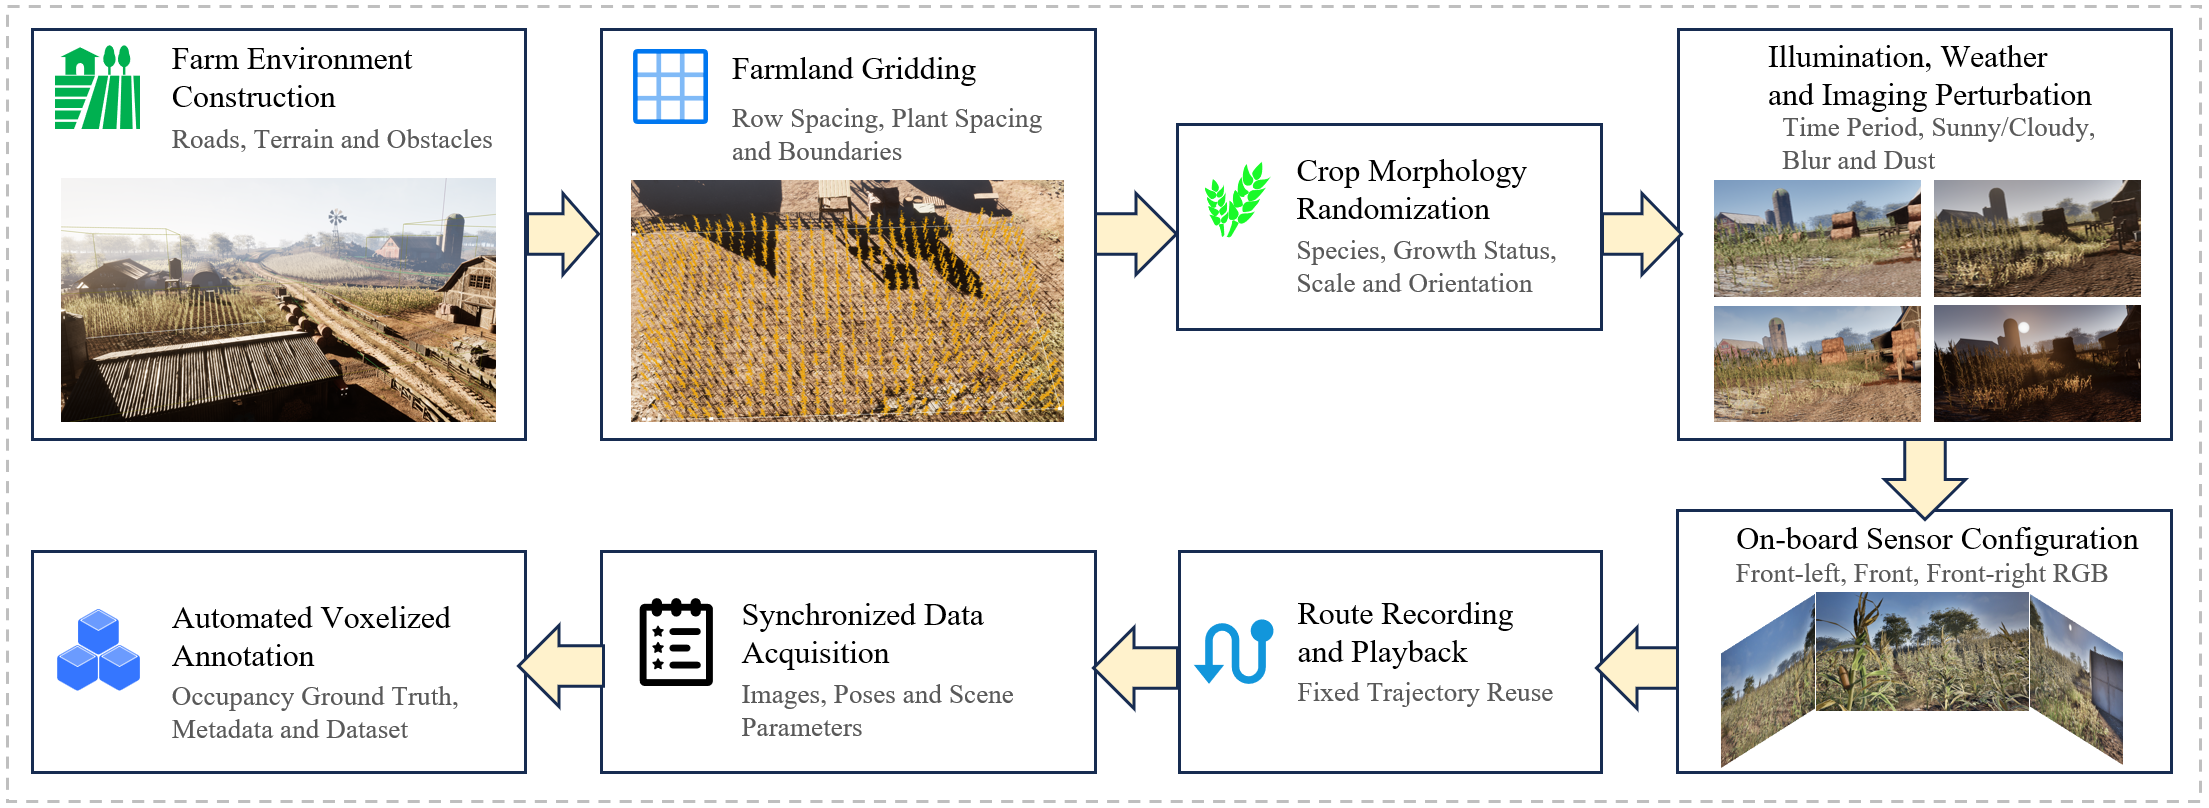
\includegraphics[width=1\linewidth]{synthetic.png}
\caption{农田仿真数据采集系统的构建流程。}
\label{fig:synthetic}
\end{figure}

采集数据时首先录制拖拉机在农田中的若干行驶轨迹，再针对不同的作物种类、生长阶段、光照时段和天气组合重放路线，
实现多样的农田场景与运动轨迹的组合。为缩小仿真与真实采集之间的外观差异，
系统进一步以设定概率在 RGB 图像上施加运动模糊、镜头污渍和扬尘颗粒等成像扰动。
数据标注方面，与 nuScenes 等真实采集数据集不同，仿真引擎可直接导出相机位姿、场景语义和体素占用状态，
无需进行人工逐帧点云语义标注、多帧点云时空配准及体素标签生成等复杂流程。
对每一帧数据，系统将车辆局部坐标系下的前方空间划分为规则三维体素网格，并基于场景几何与语义标签自动生成稠密占用真值。
原始环境语义根据任务需求归并为自由空间、作物、土壤地面、可通行区域、其他植被和其他障碍物六类，
最终，每个样本由三视角 RGB 图像、对应的三维语义占用标签以及位姿和场景参数元数据组成，从而形成可用于视觉占用预测训练与评估的农田多模态数据集。
\subsubsection{AgriOcc-Dataset}\label{sec:agriocc_dataset}
基于上述流程，我们构建了面向田间农业机器人的多视角三维语义占用数据集 AgriOcc-Dataset。
每个序列包含正前、左前和右前三视角的同步 RGB 图像、相机内外参、机器人位姿、语义占用标签及有效体素掩码。
标签在加载阶段统一映射为 free、crop、soil\_ground、drivable、other\_vegetation 和 other\_obstacle 六类，并在机器人自身坐标系中生成前方体素监督。

数据集包含 298 个仿真行驶序列，原始记录频率为 10 Hz，共约 194k 帧。
为避免相似场景大量重复，我们下采样至 2 Hz，得到 38.8k 个样本。
其中 248 个序列（32,385 帧）用于训练，50 个序列（6,477 帧）用于验证。
数据覆盖 cabbage、carrot、corn、cucumber、potato、radish、redbeet、sunflower、tomato 和 wheat 十种作物；
每种作物进一步包含 early、mid 和 mature 三个生长阶段，并覆盖 dawn、morning、noon、evening 和 night 五个时段，
以及 cloudy 与 sunny 两类天气。图\ref{fig:crop_distribution}给出了总体数据集的作物组成。

\begin{figure}[pos=htbp]
\centering
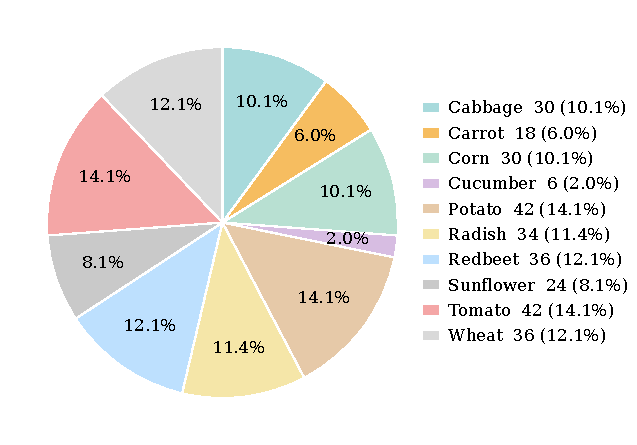
\includegraphics[width=0.5\linewidth]{crop_distribution.pdf}
\caption{AgriOcc-Dataset 的作物组成。扇区面积表示各作物的占比。}
\label{fig:crop_distribution}
\end{figure}

\begin{figure}[pos=htbp]
\centering
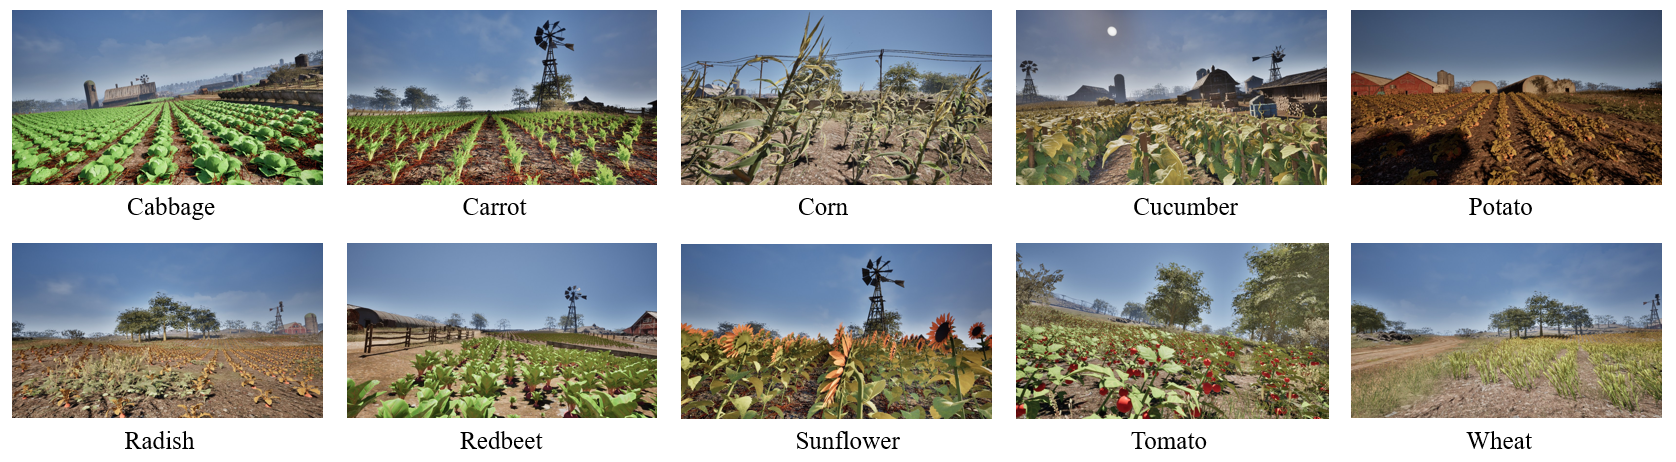
\includegraphics[width=\linewidth]{dataset.png}
\caption{AgriOcc-Dataset 中十种作物的场景示例。}
\label{fig:dataset}
\end{figure} 
 
\subsection{AgriOcc 总体结构}\label{sec:architecture}

图\ref{fig:overview}给出 AgriOcc 的总体架构。
图像编码器使用 ResNet-101 与 FPN 提取四级二维特征。
随后，六层 GeoVis-BEV 编码器以 GVAD 作为 BEV token 的上下文增强单元：在每个编码层内，
GVAD 先结合局部可变形更新与可见性引导的全局锚点，为当前 BEV 查询补充可靠的空间上下文；
再由空间交叉注意力依据相机投影关系，从多尺度图像中聚合几何对齐的视觉证据。
经逐层更新后，编码器输出 $100\times100$、通道数为 256 的 BEV token；
三层占用解码器提供多层监督，其中最后一层由 Agri-AMoE 将 BEV token 提升为
三维特征体并预测 25 个高度位置上的六类 logits。
因此，AgriOcc 利用 GVAD 优化 BEV 编码过程中的可见性驱动全局上下文建模，以近远场布局将早期编码计算聚焦于近场精细结构，并以 Agri-AMoE 自适应建模三维局部结构。

\begin{figure}[pos=htbp]
\centering

\includegraphics[width=\linewidth]{overview.png}
\caption{AgriOcc 总体结构。三路前视图像经 ResNet--FPN 提取四尺度特征；
六层 GeoVis-BEV 编码器在每层依次执行 GVAD、图像空间交叉注意力与前馈更新，
NearFar 在前五层实施近远场查询布局并在第六层前恢复稠密 BEV；三层占用解码器提供多层监督，
最后一层通过 Agri-AMoE 将 BEV token 提升为三维特征体，
并输出 $100\times100\times25\times6$ 的六类语义 logits。}
\label{fig:overview}
\end{figure}

\subsection{GeoVis-BEV 编码器}\label{sec:bev-encoder}

语义占用预测需要将有限视角下的二维视觉证据还原为机器人坐标系中的稠密三维语义空间，
但农田的作物冠层遮挡、规则而重复的行垄纹理以及前向相机的有限视场，
会使大量 BEV 单元缺乏直接或可靠的观测。由此产生的投影空洞和语义歧义，
容易造成作物--自由空间边界被过度平滑，或使弱观测区域继承错误的局部证据。
另一方面，近场作物、垄沟和障碍物的细节直接决定机器人可通行空间，远场观测则更稀疏；
对整个 BEV 平面采用统一密度和统一上下文聚合，既不能针对性补偿弱可见区域，也会浪费近场精细建模所需的计算资源。

本文以 BEVFormer 的多相机 BEV 编码框架为基础\citep{li2022bevformer}，提出 GeoVis-BEV 编码器。
它以几何投影构建局部证据、以可见性选择可靠上下文，并按任务距离配置编码预算。
该编码器在逐层图像条件更新中协同建模几何关系、观测可见性与近远场查询密度，
从而将有限的多相机观测转化为兼具局部边界与全局结构一致性的 BEV 表征。
对第 $l$ 层输入的 BEV token，编码器依次利用 GVAD 强化局部结构和可靠的长程上下文、
通过空间交叉注意力聚合几何对齐的多尺度图像特征，并经前馈网络完成表征更新；
该过程重复六次，最终输出 $100\times100$、通道数为 256 的稠密 BEV token。
 
\begin{figure}[pos=htbp]
\centering
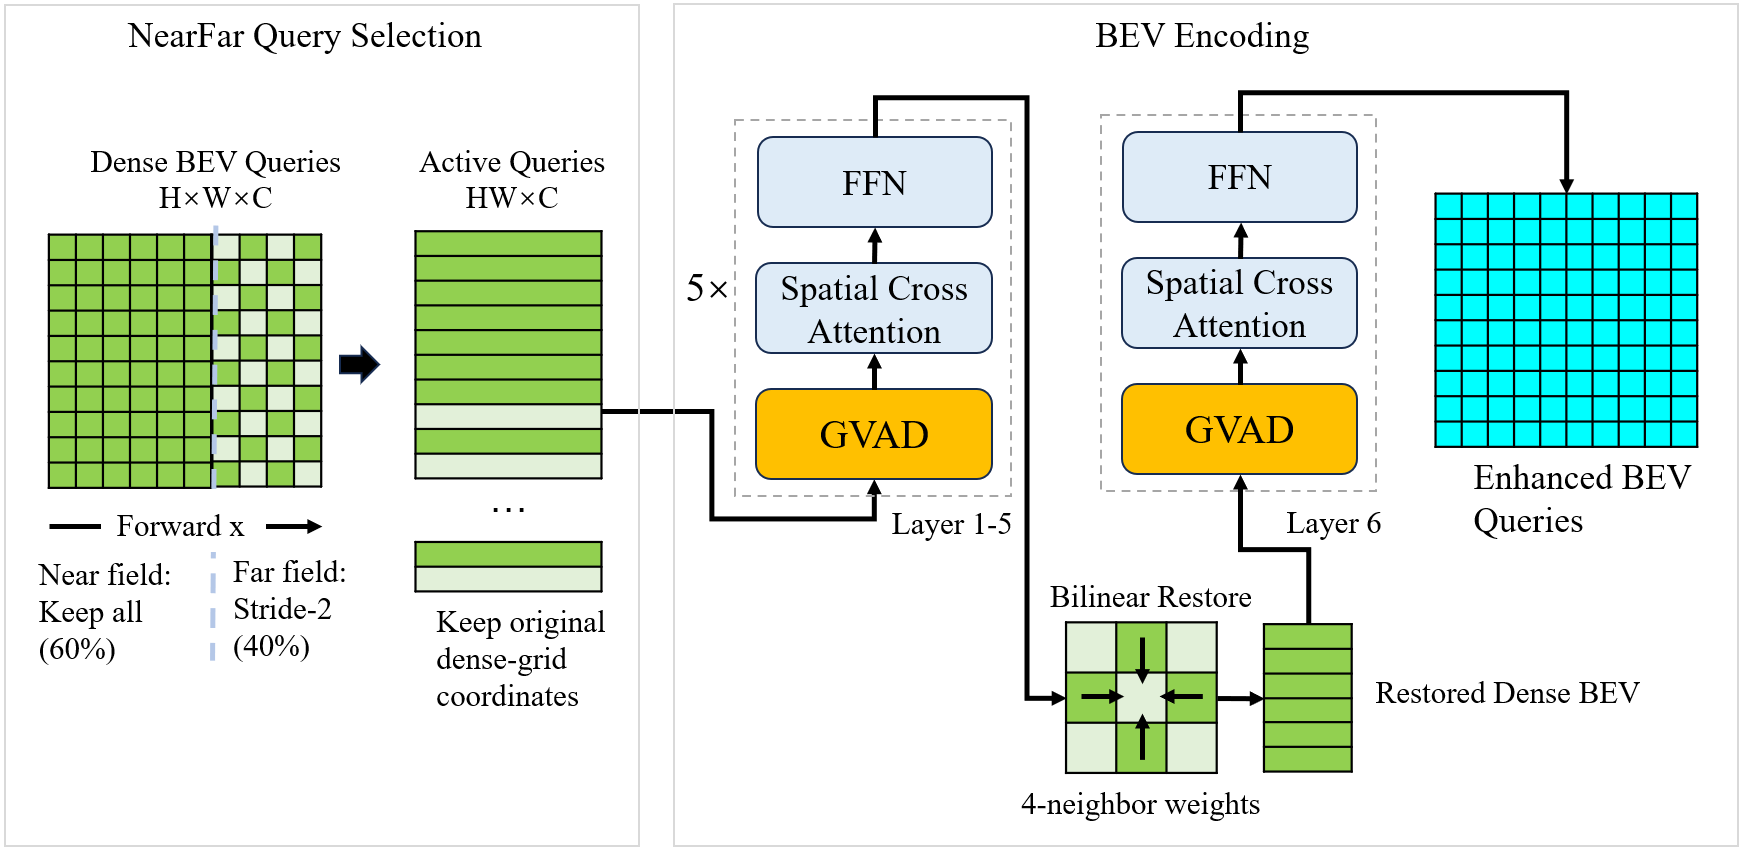
\includegraphics[width=\linewidth]{geovis-bev.png}
\caption{GeoVis-BEV 编码器整体架构。三路前视图像经 ResNet--FPN 提取多尺度特征后输入六层编码器；
GVAD 在各编码层中更新 BEV token，NearFar 在前五层保留近场稠密查询并对远场规则稀疏采样，
恢复为稠密网格后由最后一层完成图像条件细化。}
\label{fig:geovis-bev-encoder}
\end{figure}

\subsubsection{几何可见锚点可变形注意力}\label{sec:gvad}
GVAD 位于每个 GeoVis-BEV 编码层的开头，在图像空间交叉注意力之前增强 BEV 查询。
用于在保留局部投影细节的同时，按单元可见性读取可靠的长程上下文。
其输入包括第 $l$ 层的 BEV token $\bm{Q}^{l}=[\bm{q}_1,\ldots,\bm{q}_{N}]\in\R^{B\times N\times d}$、
对应的位置编码 $\bm{E}^{l}=[\bm{e}_1,\ldots,\bm{e}_{N}]$，以及由相机标定投影得到的有效掩码
$\bm{M}\in\{0,1\}^{C_{\mathrm{cam}}\times B\times N\times Z}$。
其中，$B$、$N=HW$ 和 $d$ 分别为批量大小、BEV token 数与通道维度，$H\times W$ 为 BEV 网格尺寸，
$C_{\mathrm{cam}}$ 为相机数，$Z$ 为每个 BEV 柱投影的高度参考点数。
掩码元素 $M_{c,b,i,z}=1$ 表示第 $b$ 个样本中第 $i$ 个 BEV 柱的第 $z$ 个参考点可投影至第 $c$ 个相机，
由此将多相机、多高度的投影有效性归约为 token 级可见性
\begin{equation}
m_{b,i}=\frac{1}{C_{\mathrm{cam}}Z}\sum_{c=1}^{C_{\mathrm{cam}}}\sum_{z=1}^{Z}M_{c,b,i,z}\in[0,1].
\end{equation}
后文为简洁起见省略批量索引 $b$。GVAD 首先对带位置编码的输入执行层归一化，记为
$\tilde{\bm{q}}_i=\operatorname{LN}(\bm{q}_i+\bm{e}_i)$；
随后从该表征出发并行计算局部可变形分支和几何可见锚点分支，最后以可见性门控的残差形式融合二者。
局部可变形采样继承了 BEVFormer 的查询自适应注意力骨架\citep{li2022bevformer}，
而锚点路径结合 Deformable DETR\citep{zhu2021deformable} 的稀疏聚合思想和
 DETR3D\citep{wang2022detr3d} 的几何查询机制，显式度量观测可靠性。

\paragraph{局部可变形分支。}
该分支等价于对 BEV token的可变形自注意力。
它以 $(\bm{Q}^{l},\bm{E}^{l})$ 为输入，为每个查询预测少量采样偏移与注意力权重，
并在 BEV 特征图的局部邻域内进行多头可变形聚合，得到局部更新 $\bm{d}_i$。记该操作为 $\mathcal{D}$，则
\begin{equation}
\bm{d}_i=\mathcal{D}(\bm{q}_i,\bm{e}_i)-\bm{q}_i.
\end{equation}
它保留了局部相邻 token 的结构连续性，并为随后图像空间交叉注意力提供更稳定的 BEV 查询。

\paragraph{几何可见锚点分支。}
为从可靠区域补偿弱可见查询，首先将 BEV 平面均匀划分为 $H_a\times W_a$ 个 tile；
本文取 $H_a=4$、$W_a=8$，因而得到 $K=H_aW_a=32$ 个锚点。
对于第 $a$ 个 tile 内的第 $i$ 个 token，锚点权重由内容置信度和可见性共同决定：
\begin{equation}
s_{ia}=\bm{w}_c^\top\tilde{\bm{q}}_i+\gamma\log(m_i+\epsilon),\qquad
\alpha_{ia}=\softmax_{i\in a}(s_{ia}),\qquad
\bm{z}_a=\sum_{i\in a}\alpha_{ia}\tilde{\bm{q}}_i .
\end{equation}
其中，$\bm{w}_c$ 为可学习的置信度投影，$\gamma$ 为可学习的可见性尺度，$\epsilon$ 为数值稳定常数，
$\alpha_{ia}$ 在 tile 内归一化，$\bm{z}_a\in\R^d$ 为第 $a$ 个可见锚点特征。
之后以相同权重对 token 的归一化二维 BEV 中心坐标 $\bm{r}_i\in[0,1]^2$ 加权，得到锚点坐标
$\bm{r}_a=\sum_{i\in a}\alpha_{ia}\bm{r}_i$。接着，每个查询通过带距离偏置的多头注意力读取所有锚点：
\begin{equation}
A_{i,a}^{(h)}=\frac{(W_q^{(h)}\tilde{\bm{q}}_i)^\top(W_k^{(h)}\bm{z}_a)}{\sqrt{d_h}}
-\rho_h\|\bm{r}_i-\bm{r}_a\|_2^2,\qquad
\pi_{i,a}^{(h)}=\softmax_a\left(A_{i,a}^{(h)}\right),
\end{equation}
\begin{equation}
\bm{g}_i=W_o\operatorname{Concat}_{h=1}^{H_{\mathrm{head}}}
\left(\sum_{a=1}^{K}\pi_{i,a}^{(h)}W_v^{(h)}\bm{z}_a\right).
\end{equation}
其中，$h$ 为注意力头索引，$H_{\mathrm{head}}$ 为头数，$d_h=d/H_{\mathrm{head}}$；
$W_q^{(h)}$、$W_k^{(h)}$、$W_v^{(h)}$ 和 $W_o$ 均为可学习线性投影。
$\rho_h=\operatorname{softplus}(\delta_h)\geq0$ 是第 $h$ 个头的可学习距离衰减系数，$\delta_h$ 为其无约束参数；
因此该路径允许全局读取，但优先聚合几何上较近的可靠锚点。

\paragraph{可见性门控融合。}
两分支的输出与原始查询以残差形式融合。具体地，
门控系数 $\eta_i$ 由归一化特征和 token 可见性预测，并随可见性升高而减小：
\begin{equation}
\eta_i=\sigma\left(f_g([\tilde{\bm{q}}_i,m_i])\right)(1-\beta m_i),\qquad
\bm{q}_i'=\bm{q}_i+\bm{d}_i+\eta_i\bm{g}_i,
\end{equation}
其中，$f_g$ 为可学习的门控投影，$[\cdot,\cdot]$ 表示通道拼接，$\sigma$ 为 Sigmoid 函数，
$\beta=0.75$ 为固定可见性衰减系数，$\bm{q}_i'$ 为 GVAD 输出 token。
因此，弱可见单元获得更大的锚点上下文校正，直接可见区域则以局部分支为主，避免全局信息覆盖其精细边界。
图\ref{fig:gvad} 展示了 GVAD 的双路径结构。

\begin{figure}[pos=htbp]
\centering
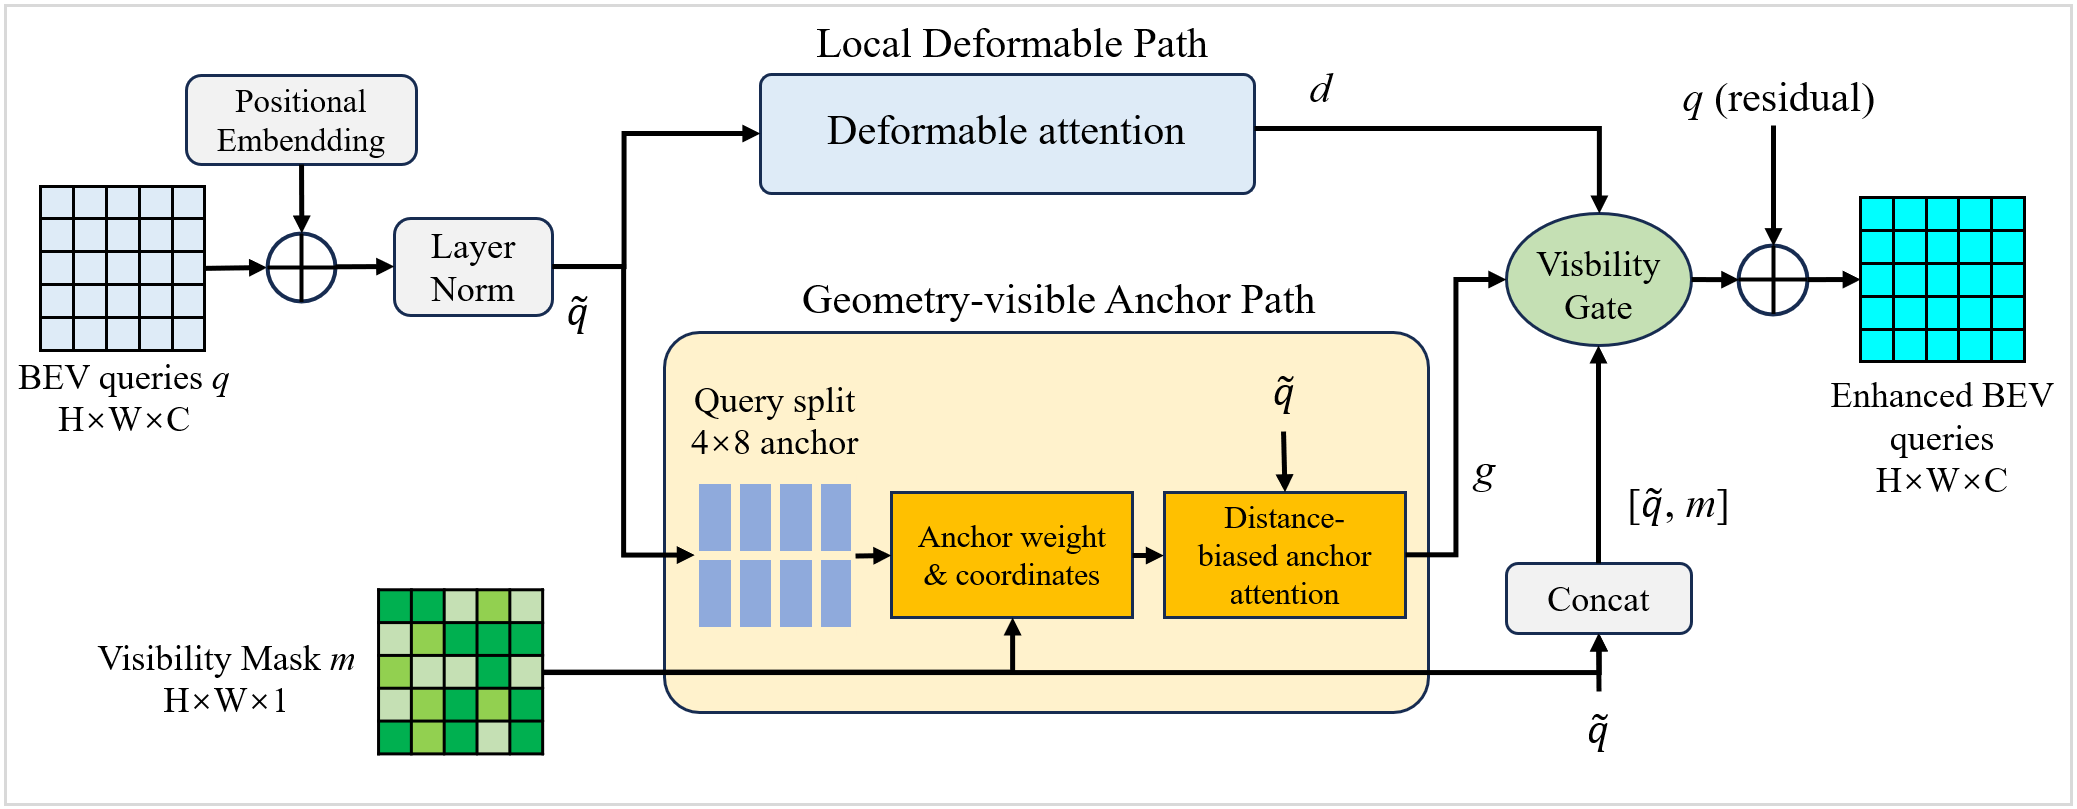
\includegraphics[width=\linewidth]{gvad.png}
\caption{GVAD 架构。相机投影掩码首先归约为每个 BEV token 的可见性；局部可变形分支根据查询预测采样位置和权重，形成局部 BEV 更新；几何可见锚点分支将 BEV 平面划分为 $4\times8$ 个 tile，以特征置信度和可见性加权构建 32 个锚点，并通过距离偏置的多头注意力形成锚点上下文。两条分支经可见性门控和残差连接融合为增强 BEV token。}
\label{fig:gvad}
\end{figure}

\subsubsection{近远场 BEV 查询布局}\label{sec:nearfar}
近远场查询布局将编码早期的计算优先分配给对规划与避障更关键、
且具有更充分图像证据的近场区域，同时保持最终占用输出为稠密网格。
沿 BEV 网格的前向距离维度（对应前向 $0$--$20\,$m），将靠近机器人的前 $60\%$ 网格
（即前向 $12\,$m 以内）划为近场，保留其全部查询；
其余 \(40\%\) 的远场网格每隔 2 个单元保留一个查询，形成二维规则稀疏采样。
前五个编码层只处理由近场稠密查询与远场稀疏查询共同构成的 active token 集合。
对于未激活的远场位置，使用其四个相邻 active token 的双线性权重恢复特征；
最后一个编码层恢复为完整 $100\times100$ 网格并执行一次稠密、图像条件的交叉注意力。
该安排避免仅由查询插值补全远场语义，同时使已有占用解码头保持不变。
GVAD 在稀疏层中仍按 token 的原始稠密 BEV 坐标分箱生成锚点，因此锚点覆盖不受稀疏采样影响。

近远场布局的架构见图\ref{fig:geovis-bev-encoder}。它保留近场的完整网格以表达作物、垄沟和障碍物的细粒度几何，同时对远场执行规则稀疏采样，并在进入最终稠密图像交叉注意力前恢复完整特征图。

 
\subsection{农业结构自适应混合专家三维占用解码器}\label{sec:agri-amoe}
农田占用空间具有显著的各向异性：作物行与垄沟在地平面上呈现长程连续和周期性交替，
作物冠层、土壤和障碍物又在高度方向具有不同的边界形态。
特别是株间空隙和作物与自由空间的边界往往只占少量体素，
若将二维 BEV token 独立地直接映射为各高度类别，
解码器难以协调相邻位置的平面细节与垂直结构，预测容易在细粒度区域发生过度平滑。
因而，最终占用头不仅需要恢复高度维度，还应按局部三维结构的复杂度自适应地选择合适的感受野与方向建模方式。

受文献\citep{shi2026oneocc}将混合专家引入占用解码的启发，本文设计农业结构自适应混合专家三维占用解码器（Agri-AMoE）。
与在通用城市场景下定义专家不同，本文依据农田空间在平面、垂直与上下文三个方向上的
各向异性结构来定义专家形态，并以可解释的梯度能量作为路由信号，
使专家分工与作物行、垄沟和冠层等农业结构直接对应。
对于最终层 BEV 特征 $\bm{Q}\in\R^{B\times HW\times C}$，先经线性映射并重排为通道数为 $C_a$ 的三维体积特征：
\begin{equation}
\bm{F}_0=\operatorname{reshape}(W_{\mathrm{lift}}\bm{Q})\in\R^{B\times C_a\times Z\times H\times W}.
\end{equation}
其中，$C$ 为输入 BEV token 的通道数，$H$、$W$ 为 BEV 网格的两个平面维度，$Z$ 为高度 bin 数，
$W_{\mathrm{lift}}$ 为可学习的 lifting 映射，$\operatorname{reshape}(\cdot)$ 仅将映射后的 token 重排为三维体积。
本文使用 $C_a=96$、$Z=25$。首先，对 $\bm{F}_0$ 进行全局三维池化，并经MLP生成通道注意力权重，以增强三维体积特征：
\begin{equation}
\bm{F}=\bm{F}_0\odot\sigma\!\left(f_c(\operatorname{GAP}(\bm{F}_0))\right).
\end{equation}
其中，$\operatorname{GAP}$ 表示在 $Z$、$H$、$W$ 维度上的全局平均池化，$f_c$ 为可学习的通道映射，
$\sigma$ 为 Sigmoid 函数，$\odot$ 为逐元素乘法。增强后的 $\bm{F}$ 被同时送入三个并行的各向异性专家和路由分支。
三个专家均以 $\bm{F}$ 为输入：$\mathcal{E}_1$ 采用 $1\times3\times3$ 深度可分离卷积编码株间平面细节，
$\mathcal{E}_2$ 采用 $3\times1\times1$ 卷积编码垂直结构，$\mathcal{E}_3$ 则采用膨胀率为 2 的 $1\times3\times3$ 卷积编码较大范围的平面上下文。

随后，路由器根据 $\bm{F}$ 的空间显著性与局部结构变化，为每个体素分配专家权重。
空间显著性由 $\bm{F}$ 的通道均值和最大值经 $3\times3\times3$ 卷积空间映射 $f_s$ 得到：
\begin{equation}
\bm{S}=\sigma\!\left(f_s([\operatorname{mean}_c(\bm{F}),\operatorname{max}_c(\bm{F})])\right).
\end{equation}
其中，$\operatorname{mean}_c$ 与 $\operatorname{max}_c$ 分别表示沿通道维度的平均与最大聚合，$\bm{S}$ 为逐体素空间显著性图。
为使专家选择进一步与三维结构复杂度对齐，路由器还计算 $\bm{F}$ 在三个空间方向的有限差分能量：
\begin{equation}
\bm{E}=\operatorname{mean}_c\!\left((\nabla_x\bm{F})^2+(\nabla_y\bm{F})^2+(\nabla_z\bm{F})^2\right).
\end{equation}
其中，$\nabla_x$、$\nabla_y$ 和 $\nabla_z$ 分别为三个空间方向的梯度，故 $\bm{E}$ 为逐体素的局部结构变化强度。
路由器以 $[\log(1+\bm{E}),\bm{S}]$ 为输入，在温度 $\tau=1$ 下输出三个归一化专家权重：
\begin{equation}
\bm{\alpha}=\operatorname{Softmax}\!\left(g([\log(1+\bm{E}),\bm{S}]) / \tau\right),
\end{equation}
其中，$g$ 为由两层 $1\times1\times1$ 卷积、组归一化和 ReLU 构成的三路由映射，
$\alpha_k$ 为第 $k$ 个专家在每个体素处的权重。最后，路由权重用于融合三个已计算的专家输出：
\begin{equation}
\bm{F}'=\operatorname{ReLU}\!\left(\bm{F}+\operatorname{GN}\!\left(\sum_{k=1}^{3}\alpha_k\mathcal{E}_k(\bm{F})\right)\right),\qquad
\bm{O}=W_o\bm{F}',
\end{equation}
其中，$\operatorname{GN}$ 为组归一化，$\operatorname{ReLU}$ 为非线性激活，$W_o$ 为 $1\times1\times1$ 分类卷积，
$\bm{O}\in\R^{B\times6\times Z\times H\times W}$ 为最终语义 logits。图\ref{fig:agri-amoe}展示了该模块的架构。
\begin{figure}[pos=htbp]
\centering
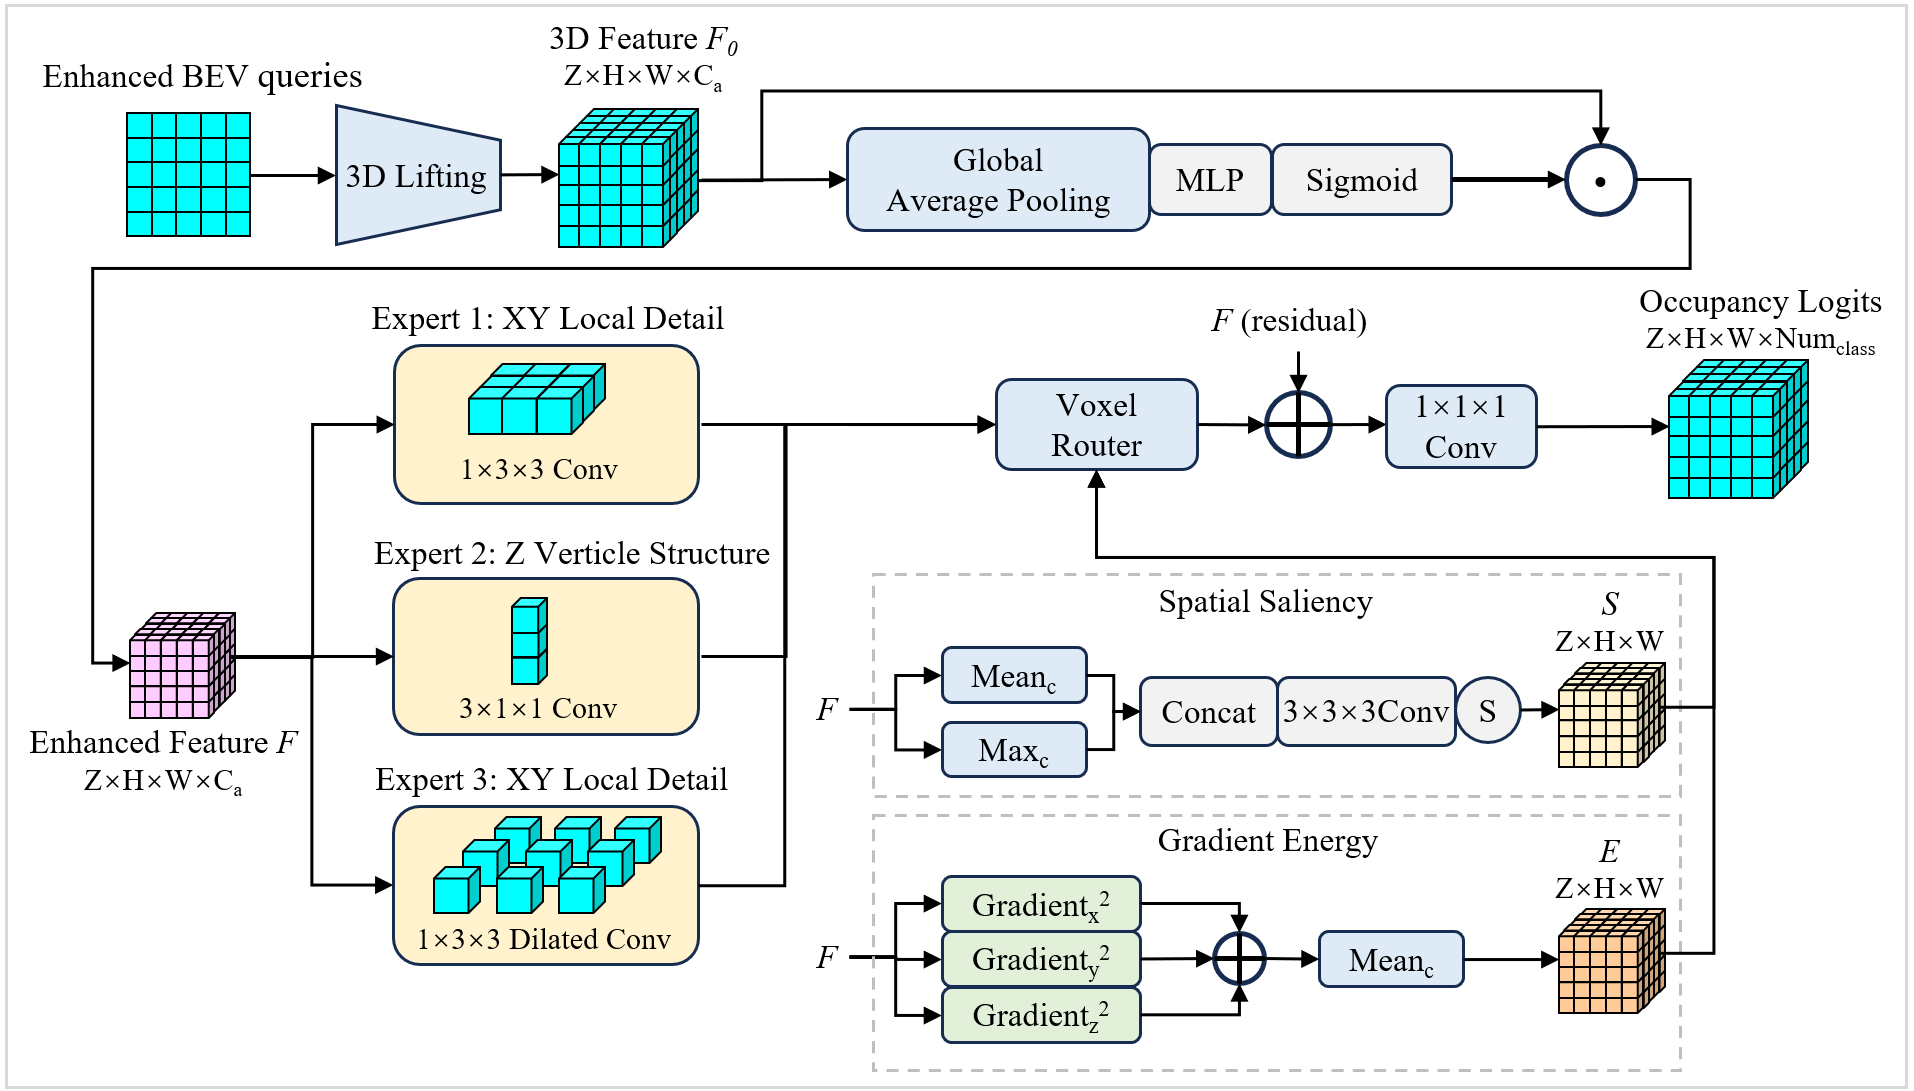
\includegraphics[width=\linewidth]{agri-amoe.png}
\caption{Agri-AMoE 三维占用解码器。二维 BEV token 经 lifting 形成三维体积，并首先由通道注意力增强；增强特征一方面并行输入三个各向异性专家，另一方面生成空间显著性与三方向梯度能量以计算逐体素路由权重。三个专家输出经加权求和与残差融合后完成最终分类。}
\label{fig:agri-amoe}
\end{figure}

\subsection{总体优化目标}\label{sec:loss}
占用主损失遵循 SurroundOcc 与 OpenOccupancy 的多层体素监督范式\citep{wei2023surroundocc,wang2023openoccupancy}，
由类别交叉熵、语义尺度损失、几何尺度损失和 Lov\'{a}sz-Softmax 项组成；其具体计算与上述工作一致，故不再重复推导。

\section{实验}\label{sec:experiments}

\subsection{数据集与评价协议}\label{sec:data}
\paragraph{AgriOcc-Dataset}
我们的绝大部分实验在 AgriOcc-Dataset 上完成，其构建过程见第\ref{sec:dataset_construction}节。
AgriOcc 使用正前、左前和右前三路相机，预测机器人前方 $20\,\mathrm{m}\times20\,\mathrm{m}$
区域（横向 $\pm10\,$m）的占用。

\paragraph{ORAD-3D}
另外，为测试仿真到真实环境的迁移，我们在\ref{sec:sim2real}节使用 ORAD-3D 数据集\citep{chen2025orad3d}评估AgriOcc在真实野外和农田占用预测任务中的性能。

\paragraph{指标}
我们用mIoU和每个类别的IoU来评价语义占用模型的性能。对类别 $c$，$\IoU_c=\mathrm{TP}_c/(\mathrm{TP}_c+\mathrm{FP}_c+\mathrm{FN}_c)$；
mIoU 为有效类别 IoU 的算术均值。

\subsection{实现细节}\label{sec:implementation}
AgriOcc 采用在 ImageNet 上预训练的 ResNet-101 作为图像编码器，并使用 6 层 GeoVis-BEV 编码器与 3 层占用解码器。
输入图像尺寸为 $512\times288$；
体素范围为 $[0,20]\times[-10,10]\times[-2,3]\,\mathrm{m}$，分辨率 $0.2\,\mathrm{m}$。
优化器为 AdamW，初始学习率 $2\times10^{-4}$，权重衰减 $0.01$，采用余弦学习率策略与
500 次迭代的线性 warm-up，有效全局 batch size 为 24，
使用 4 张 RTX 4090 GPU 训练 8 个 epoch。

\subsection{与现有方法的比较}\label{sec:comparison}
表\ref{tab:main}汇总 AgriOcc-Dataset 上的占用预测结果对比。
SurroundOcc\citep{wei2023surroundocc}、SparseOcc\citep{tang2024sparseocc}与 COTR\citep{ma2024cotr}同属当前帧语义占用方法；
Drive-OccWorld\citep{yangDrivingOccupancyWorld2025}和 IR-WM\citep{meiVisionCentric4DOccupancy2026}则同时预测当前与未来占用。
结果表明，AgriOcc 优于各对比方法。说明 GeoVis-BEV 编码器与
农业结构自适应解码器能够将图像几何线索转化为更一致的空间占用表示。
优势主要体现在地面、可通行区域和复杂植被/障碍物等结构性类别，
表明模型对大范围农田布局与局部障碍边界具有更稳健的联合建模能力。
相比之下，作物仍是最具挑战性的类别，原因在于株间分离和叶片遮挡会在单帧投影及体素化过程中造成语义混合；
这也为后续引入更细粒度时空观测提供了明确的方向。

SurroundOcc、SparseOcc 和 COTR 的设计主要面向城市环视驾驶场景：均匀的空间查询与城市道路先验难以直接适配农业机器人前方视域中的行间遮挡、细长作物和近场精细边界。相比之下，IR-WM 与 Drive-OccWorld 的重点是利用历史状态、动作条件和未来滚动预测服务于世界建模与规划；在本文仅评价当前帧占用的协议下，这些额外能力无法充分转化为当前体素精度，且多步联合优化会增加表征学习的难度。因此，它们较低的当前帧指标反映了任务目标与模型归纳偏置的不匹配，而非世界模型在预测未来状态或规划任务中的能力不足。

\begin{table}[pos=htbp]
\centering
\caption{AgriOcc-Dataset 验证集上的三维语义占用结果（\%）。
参数量为训练时的可训练参数量；其中 SurroundOcc、SparseOcc 与 COTR 为当前帧语义占用方法，
Drive-OccWorld 与 IR-WM 为同时预测未来占用的世界模型方法，本文仅比较其当前帧输出。}
\label{tab:main}
\fontsize{9}{11}\selectfont
\setlength{\tabcolsep}{2.6pt}
\begin{threeparttable}
\begin{tabular}{lrrrrrrrr}
\toprule
方法 & 参数(M) & mIoU & Free & Crop & Soil & Drivable & Other veg. & Other obs. \\
\midrule
SurroundOcc & 222.38 & 50.50 & 88.95 & 25.20 & 63.44 & 58.92 & 36.79 & 29.69 \\
SparseOcc & 58.14 & 37.10 & 83.53 & 17.66 & 38.99 & 34.02 & 25.82 & 22.31 \\
COTR & 37.17 & 36.50 & 91.11 & 8.59 & 54.48 & 30.88 & 26.50 & 7.42 \\
Drive-OccWorld & 60.68 & 35.15 & 85.52 & 19.63 & 40.29 & 29.64 & 21.06 & 14.77 \\
IR-WM & 60.68 & 35.15 & 85.52 & 19.63 & 40.29 & 29.66 & 21.06 & 14.76 \\
\midrule
\textbf{AgriOcc} & \textbf{55.74} & \textbf{56.99} & \textbf{91.11} & \textbf{28.82} & \textbf{74.03} & \textbf{68.27} & \textbf{43.57} & \textbf{36.15} \\
\bottomrule
\end{tabular}
\end{threeparttable}
\end{table}

图\ref{fig:qualitative_comparison}给出了三个具有代表性的农田场景的定性比较。
AgriOcc 对作物行、地面边界和远近区域的语义布局保持了更好的空间连续性，并能更稳定地保留局部障碍物结构。
\begin{figure}[pos=htbp]
\centering
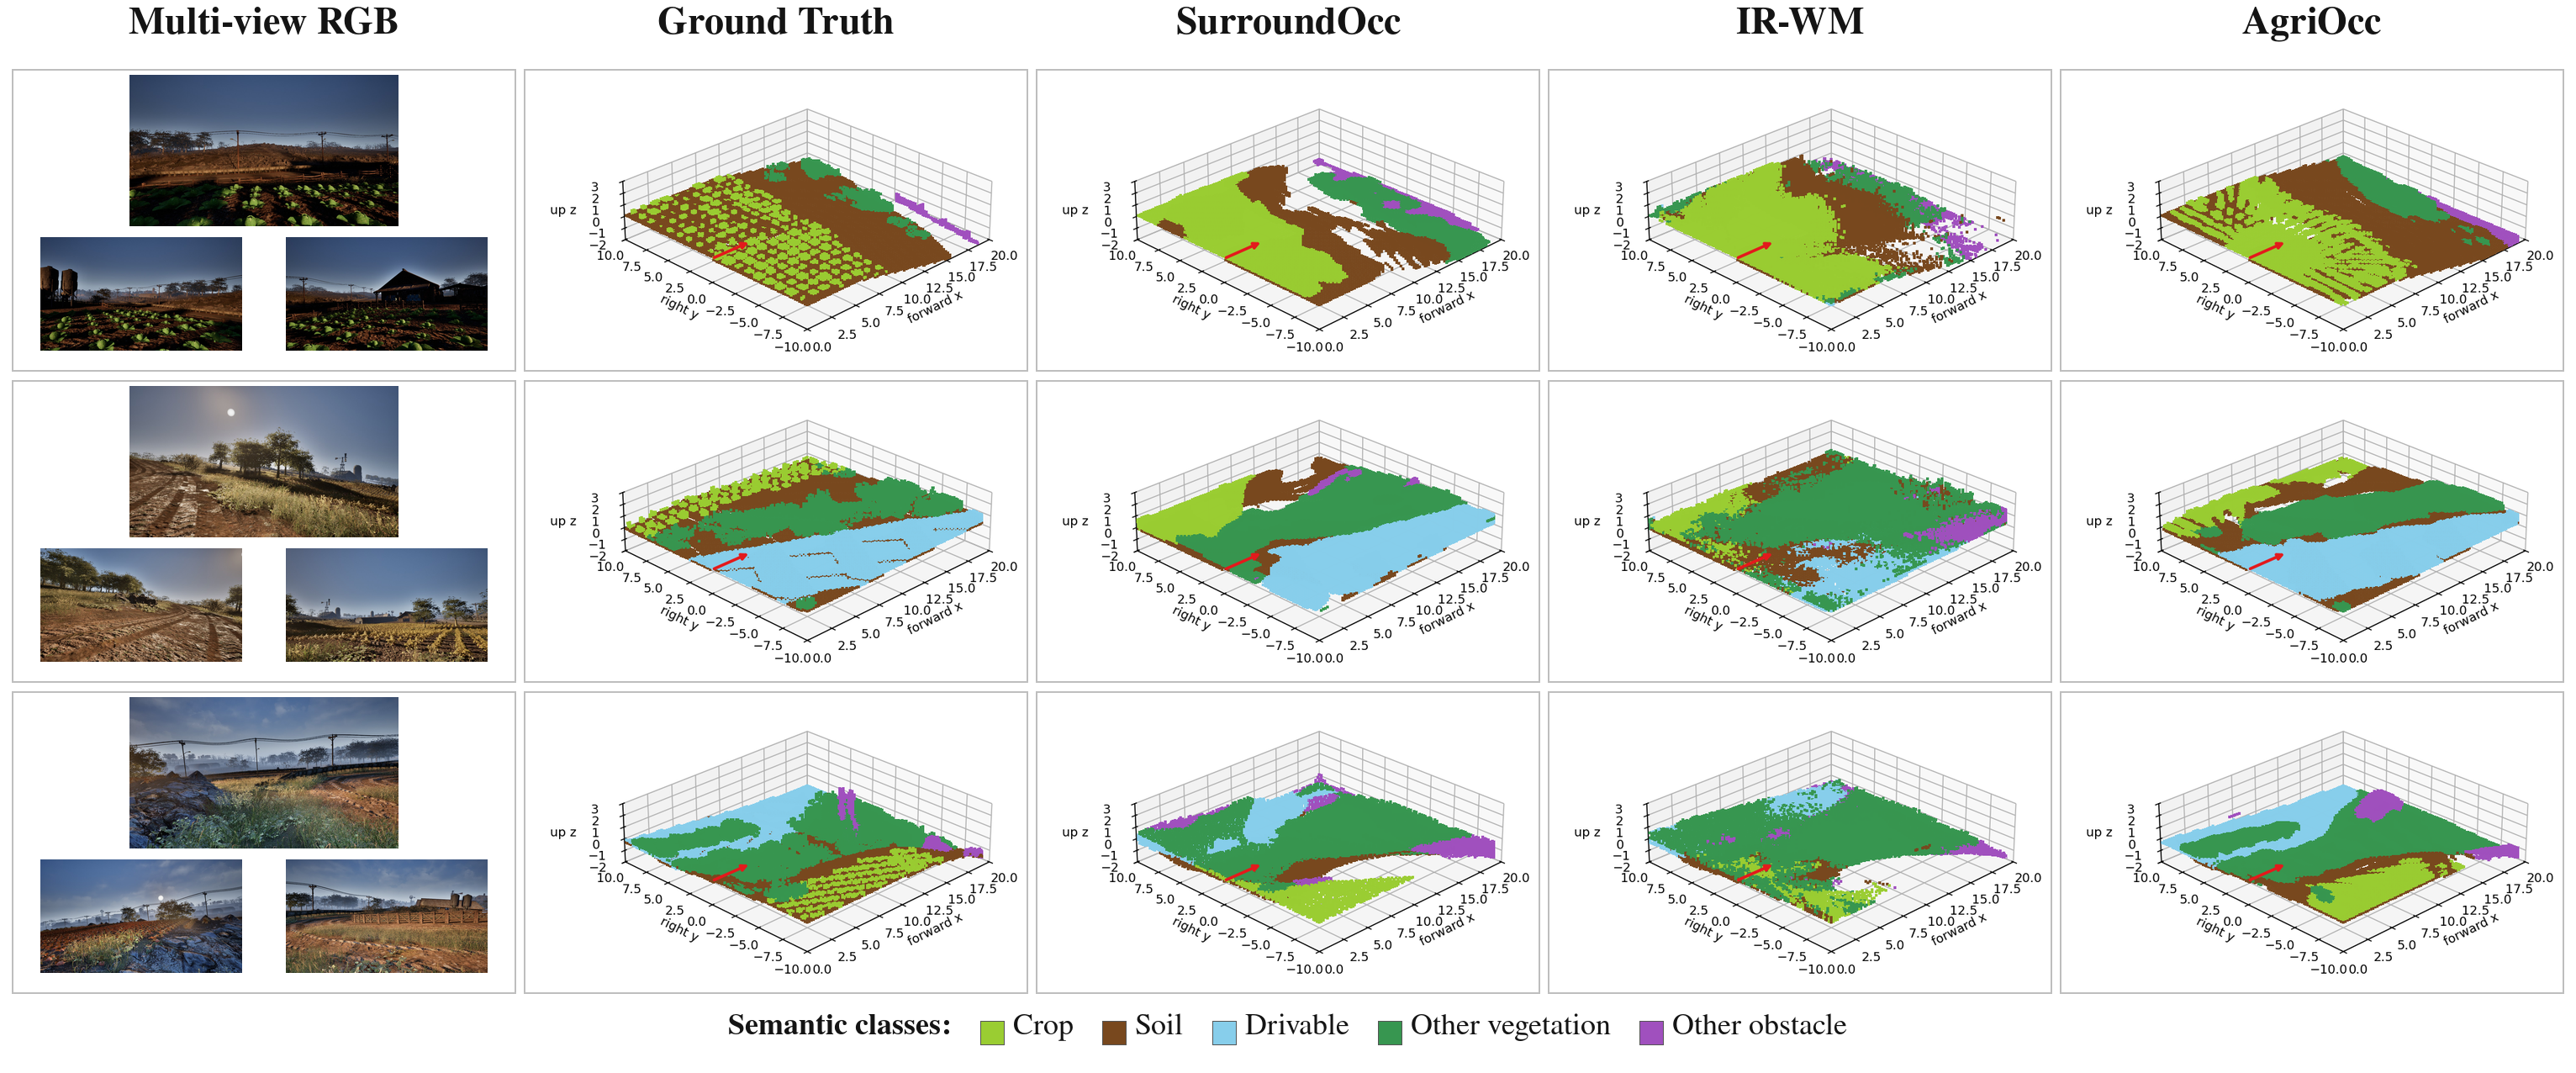
\includegraphics[width=\linewidth]{qualitative_comparison_3x5.png}
\caption{AgriOcc-Dataset 上的定性比较。每一行对应一个不同作物、光照和场景条件下的样本；从左至右依次为三路输入 RGB 图像、真值标签、SurroundOcc、IR-WM 和 AgriOcc 的当前帧三维语义占用预测。图中红色箭头为行驶方向。}
\label{fig:qualitative_comparison}
\end{figure}

\subsection{消融实验}\label{sec:ablation}
表\ref{tab:ablation}按模块的累积方式验证各设计的作用，四组配置均在相同数据划分与训练预算下运行。
GVAD 的加入带来最明显的增益（53.89\% → 56.24\%），
表明以可见锚点约束 BEV 查询能够缓解农业场景中由遮挡和视角变化引起的几何歧义。
在此基础上加入 NearFar 后 mIoU 为 56.49\%，提升幅度较小（+0.25），
但在显存与训练吞吐上收益明确，说明任务受益于与机器人作业范围相匹配的空间采样布局，
且该模块的主要价值在于计算分配而非精度本身。
进一步加入 Agri-AMoE 后达到 56.99\%，说明 Agri-AMoE 与几何编码、近远场查询互补：
前者自适应选择三维局部与上下文表征，后两者提供稳定的 BEV 输入。

NearFar 的计算收益还体现为训练吞吐与显存占用。在每卡 batch size 为 2 的测量条件下，
加入 NearFar 后单卡峰值显存由 15.14\,GB 降至 10.68\,GB（相对 +\,GVAD 配置减少 29.5\%），
训练时间减少 13.1\%。这说明远场稀疏查询降低了每个有效 batch 的总体编码开销，
并允许在相同显存下使用更大的微批。
由于两组的参数量几乎相同（55.08M 与 55.12M），该收益主要归因于查询数量的下降。
 
\begin{table}[pos=htbp]
\centering
\caption{AgriOcc-Dataset 消融实验。\checkmark 表示对应模块启用。训练时间由第 8 轮平均迭代时间与每轮迭代数估算；
所有配置均采用 4 张 RTX 4090 和有效全局 batch size 为 24。显存为固定每卡 batch size 为 2、
一次预热后前向--反向传播测得的单卡峰值分配显存。}
\label{tab:ablation}
\fontsize{9}{11}\selectfont
\setlength{\tabcolsep}{1.4pt}
\begin{tabular}{lccccccr}
\toprule
配置 & GVAD & NearFar & Agri-AMoE & 参数(M) & 显存(GB) & 训练(min/epoch) & mIoU(\%) \\
\midrule
Base  &  &  &  & 52.12 & 13.08 & 26.02 & 53.89 \\
+ GVAD & \checkmark &  &  & 55.08 & 15.14 & 42.93 & 56.24 \\
+ NearFar & \checkmark & \checkmark &  & 55.12 & \textbf{10.68} & 37.28 & 56.49 \\
+ Agri-AMoE & \checkmark & \checkmark & \checkmark & \textbf{55.74} & 11.03 & 40.95 & \textbf{56.99} \\
\bottomrule
\end{tabular}
\end{table}

\subsection{仿真到真实越野场景迁移}\label{sec:sim2real}
为了进一步验证仿真数据集上训练的模型在真实世界的有效性，本节我们在 ORAD-3D 数据集\citep{chen2025orad3d}上
对 AgriOcc-Dataset 上训练好的 AgriOcc checkpoint 进行迁移学习，并评估其官方测试集和农田子集上的性能。
ORAD-3D 的占用预测网格形状为 $100\times100\times16$，共有九类体素，类别定义沿用其官方标注协议。
AgriOcc 的输入接口按三路前视相机设计，与 ORAD-3D 提供的环视传感器配置不匹配，
且两者的类别体系也不相同，因此本文只取中心前视相机的 BEV embedding，
替换为适配目标网格形状与类别数的占用头，再使用 ORAD-3D 训练集进行对齐训练。

我们使用在 AgriOcc-Dataset 上预训练的模型进行目标域适配，并与从头训练的 AgriOcc 模型和 ORAD-3D 论文中的基准模型进行比较。
表\ref{tab:orad}同时给出 ORAD-3D 官方测试集和从中筛选出的农田场景子集的结果。
\texttt{Test} 在完整类别上计算，\texttt{Test\_farm} 则按农田子集中出现的类别计算。
为与 ORAD-3D 论文中的语义 mIoU 保持可比，表中额外报告去除 Free 类后的 Test mIoU。
表中OpenOcc、OccFormer 和 SurroundOcc 的结果引自 ORAD-3D 论文\citep{chen2025orad3d}。
结果表明，在相同的完整目标域训练数据下，AgriOcc-Dataset 预训练后仅需 2 个 epoch 的适配，
即可在 \texttt{Test (w/o Free)} 上达到 11.17\%，高于从头训练的 9.01\% 与 ORAD-3D 论文中报告的 7.60\%，
同时将目标域训练时间由 54.1 分钟降至 18.5 分钟。
这说明仿真农业数据预训练获得的图像--BEV 几何与三维语义先验能够有效迁移到真实越野场景，
从而以更低的目标域适配成本提升语义占用预测性能。


\begin{table}[pos=htbp]
\centering
\caption{ORAD-3D 仿真到真实迁移结果（\%）。两组 AgriOcc 均使用完整 ORAD-3D 训练集，
并仅使用中心前视相机输入；迁移模型以 AgriOcc-Dataset 预训练权重初始化后进行 2 个 epoch 适配。
\texttt{Test (w/o Free)} 为去除 Free 类别后的 mIoU，与 ORAD-3D 论文口径一致；
\texttt{Test} 为全部九类的 mIoU；\texttt{Test\_farm} 为农田场景子集上按出现类别计算的 mIoU。
OpenOcc、OccFormer 与 SurroundOcc 的结果引自 ORAD-3D 论文.}
\label{tab:orad}
\fontsize{9}{11}\selectfont
\setlength{\tabcolsep}{2.6pt}
\begin{tabular}{lrrrr}
\toprule 
方法 & 训练时间(min) & Test (w/o Free) & Test & Test\_farm \\
\midrule
OpenOcc\citep{jiang2024openocc} & -- & 5.83 & -- & -- \\
OccFormer\citep{zhang2023occformer} & -- & 7.45 & -- & -- \\
SurroundOcc\citep{wei2023surroundocc} & -- & 7.60 & -- & -- \\
\midrule
AgriOcc（从头训练） & 54.1 & 9.01 & 18.16 & 31.83 \\
\midrule
AgriOcc（预训练迁移） & 18.5 & \textbf{11.17} & \textbf{20.11} & 39.45 \\
\bottomrule
\end{tabular}
\end{table}
 
图\ref{fig:orad_qualitative}进一步在三个 ORAD-3D 官方测试样本上比较真值、从头训练和使用全部 ORAD-3D 训练数据迁移后的预测结果。
\begin{figure}[pos=htbp]
\centering
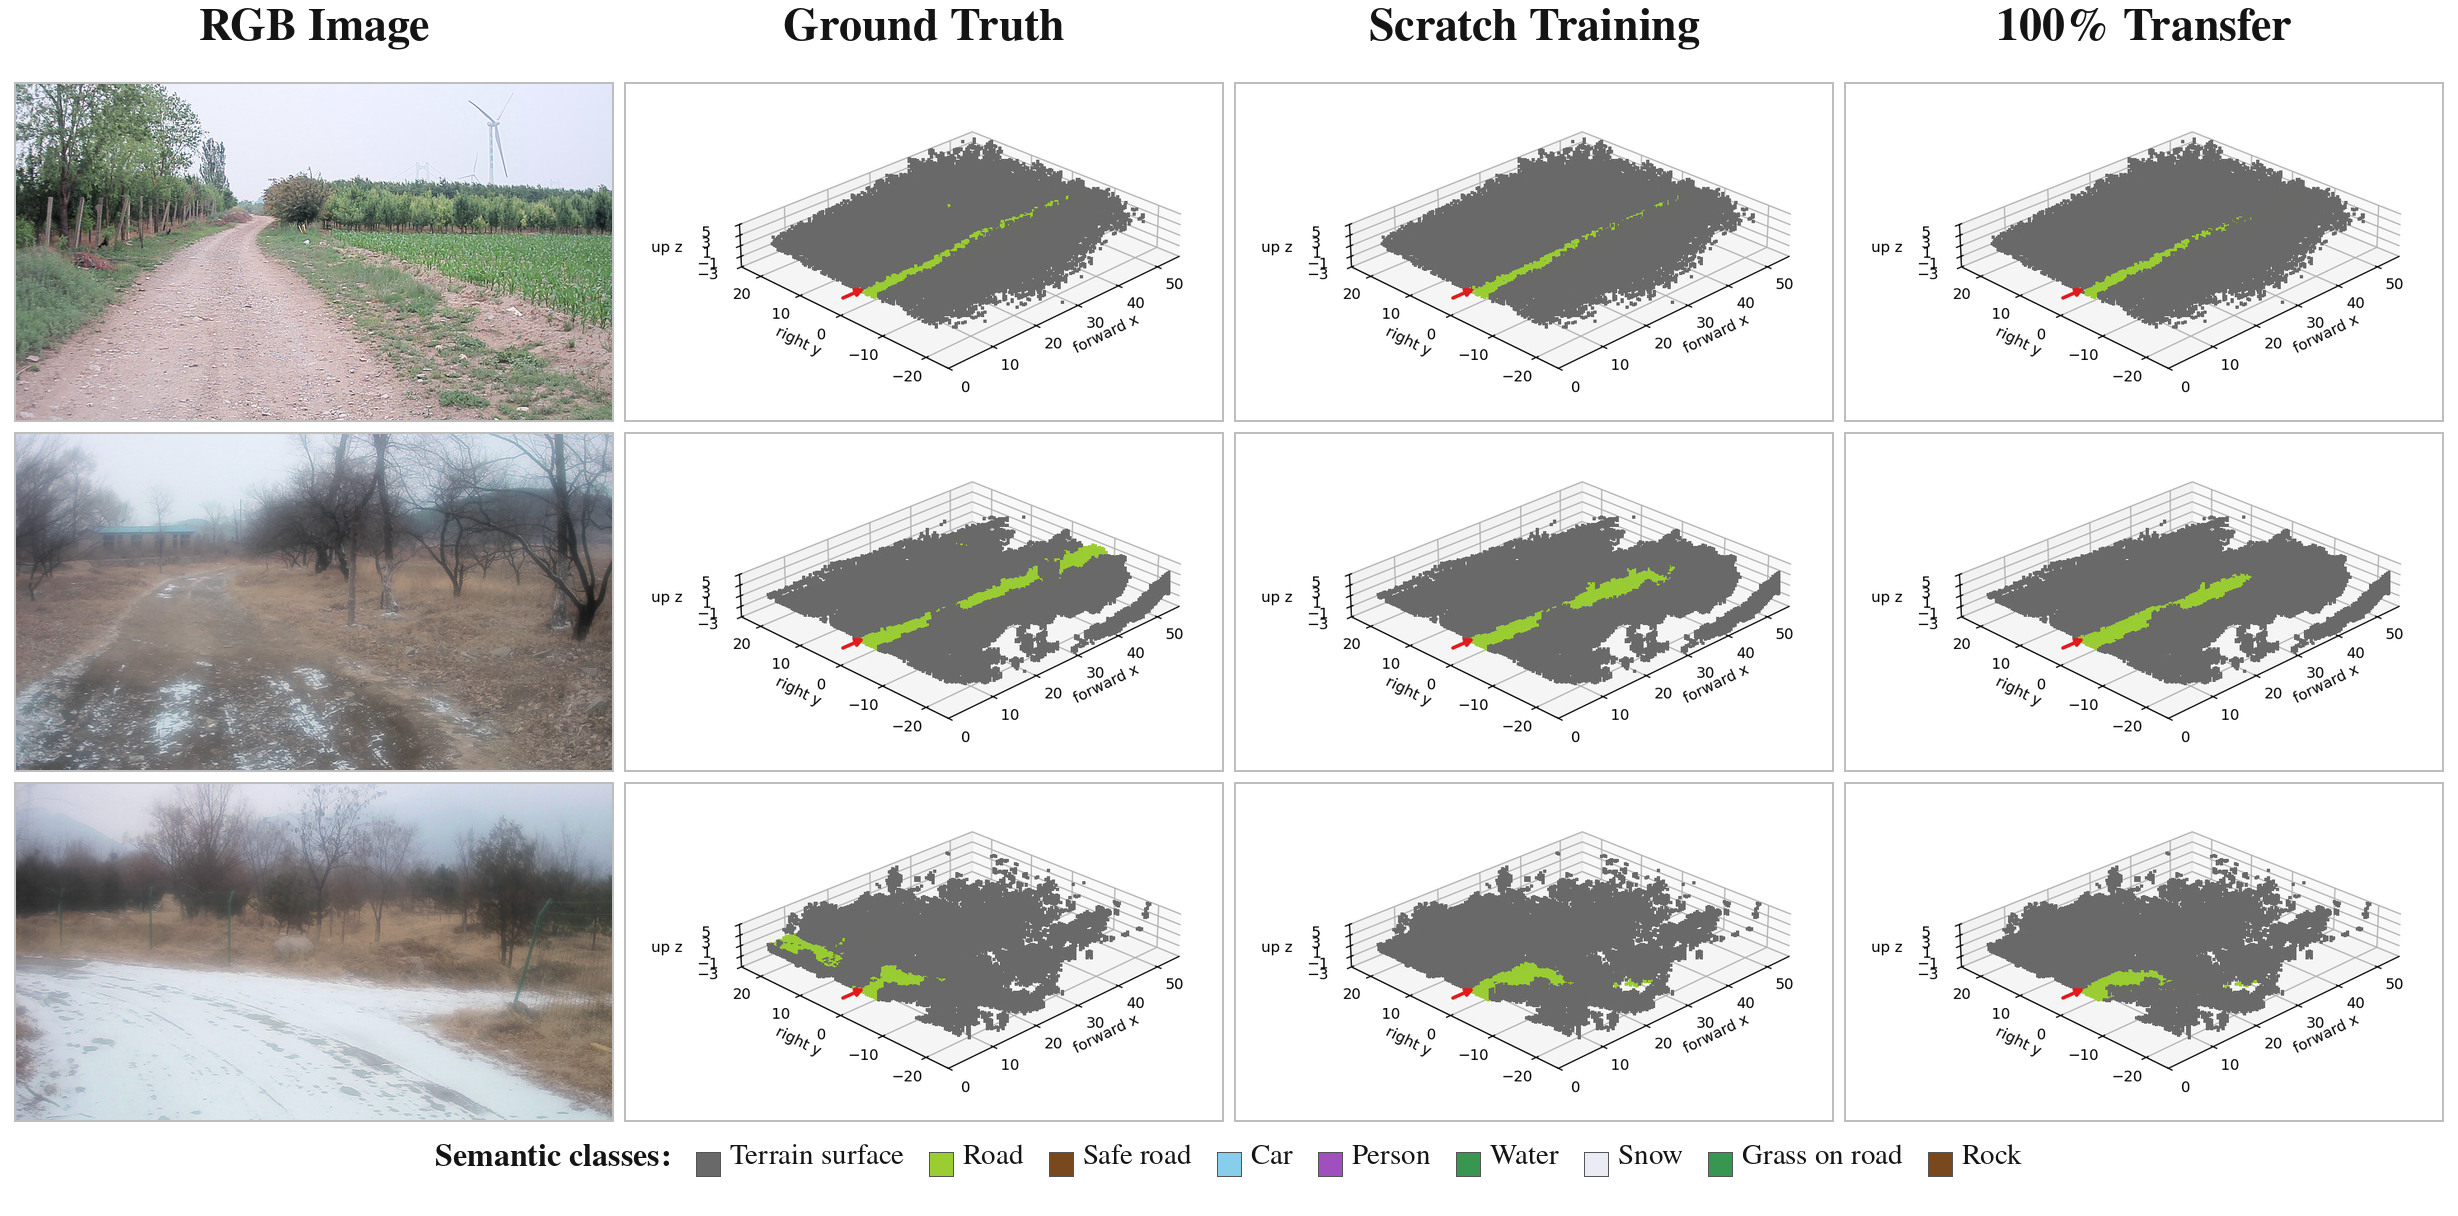
\includegraphics[width=\linewidth]{orad3d_transfer_qualitative.png}
\caption{ORAD-3D 上的定性迁移比较。每行对应同一官方测试样本；从左至右为输入 RGB 图像、真值标签、使用全部 ORAD-3D 训练数据的从头训练结果，以及 AgriOcc-Dataset 预训练后在全部 ORAD-3D 训练数据上迁移的结果（100\% Transfer）。}
\label{fig:orad_qualitative}
\end{figure}

\subsection{体素分辨率迁移}\label{sec:resolution_transfer}
本文构建的 AgriOcc-Dataset 的体素分辨率为 $0.2\,\mathrm{m}$，与主流自动驾驶语义占用基准一致\citep{behley2019semantickitti,li2024sscbench}。
但是农业机器人在垄间通行、株间避障和精细作业时，$0.2\times0.2\times0.2\,\mathrm{m}$ 的体素可能将相邻作物、
窄垄沟或局部可通行边界量化到同一网格中，带来潜在的精度不足问题。
然而，将整个 BEV 编码器直接扩展到 $0.1\times0.1\times0.2\,\mathrm{m}$ 会使
XY 查询数从 $100\times100$ 增至 $200\times200$，即增加四倍；
相应地，多尺度图像--BEV 交互、BEV 中间激活和三维占用监督的计算与显存开销均显著上升。
为此，我们另外采集了一个 $0.1\times0.1\times0.2\,\mathrm{m}$ 分辨率的小型仿真数据集，
包含 19,300 个样本，并按 1:1 划分为训练集和验证集。
我们使用它来进一步验证 AgriOcc 是否能够将已学习的标准分辨率三维先验高效迁移到细分辨率占用预测。

具体地，迁移模型首先在 $0.2\times0.2\times0.2\,\mathrm{m}$ 的 AgriOcc-Dataset 上完成训练，
保留其 $100\times100$ 的 GeoVis-BEV 编码器与 Agri-AMoE 解码器；
随后在 $0.1\times0.1\times0.2\,\mathrm{m}$ 数据上微调，并在占用输出端加入学习式 $2\times$ 细化头。
该头将粗占用 logits 与相应的 BEV 特征投影融合，输出 $200\times200\times25$ 体素。
对照组则在同一个$0.1\,\mathrm{m}$分辨率数据集上从头训练，直接学习 $200\times200$ 的高分辨率 BEV 与占用预测；
两组结果如表\ref{tab:resolution_transfer}所示。

\begin{table}[pos=htbp]
\centering
\caption{$0.1\,\mathrm{m}$ 体素分辨率的迁移结果（\%）。
迁移方法先在 $0.2\times0.2\times0.2\,\mathrm{m}$ 数据上训练，再适配至 $0.1\times0.1\times0.2\,\mathrm{m}$；
对照组在同一个$0.1\,\mathrm{m}$分辨率数据集上从头训练，直接学习 $200\times200$ 的高分辨率 BEV 与占用预测。}
\label{tab:resolution_transfer}
\fontsize{9}{11}\selectfont
\setlength{\tabcolsep}{2.4pt}
\begin{tabular}{lrrrrrrr}
\toprule
方法 & mIoU & Free & Crop & Soil & Drivable & Other veg. & Other obs. \\
\midrule
0.1 m 从头训练 & 36.18 & 89.27 & 16.74 & 52.92 & 20.11 & 23.45 & 14.56 \\
\midrule
\textbf{0.2 m 预训练 $\rightarrow$ 0.1 m 细化} & \textbf{49.01} & \textbf{92.39} & \textbf{22.61} & \textbf{73.75} & \textbf{44.29} & \textbf{35.49} & \textbf{25.50} \\
\bottomrule
\end{tabular}
\end{table}

表\ref{tab:resolution_transfer}显示，预训练迁移在所有语义类别上均优于直接高分辨率训练，
且对地面和可通行区域等连续结构的改善尤为明显。这说明 $0.2\,\mathrm{m}$ 预训练学习到了
可复用的图像--BEV 投影关系、可见性约束与场景级语义布局。
因而，微调阶段可以将有限的高分辨率监督集中用于恢复局部边界、垄沟与作物间隙，
而不必重新估计相机几何和大范围田间结构。

从优化角度看，直接高分辨率训练必须同时学习四倍数量的 BEV 查询及其图像对应关系；
在训练样本规模不变时，每个高分辨率体素获得的有效几何观测更稀疏，
迁移方案保留 $100\times100$ 编码器的稳定全局上下文，并以残差式 $2\times$ 输出细化将粗预测上采样到 0.1 m 网格。
因而，细化头只需学习粗网格未表达的高频空间残差，而不必重建完整的三维场景；
这解释了其在作物、地面和可通行区域上的一致增益，也说明 AgriOcc 能在不承担端到端高分辨率 BEV 编码成本的条件下适配精细农业感知需求。

\subsection{讨论与局限性分析}\label{sec:discussion}
AgriOcc 的总体增益集中于地面、可通行区域和复杂背景类别，说明可见性建模、
三维结构自适应解码和近远场计算分配能够提升农业场景的大范围空间一致性。
Agri-AMoE 通过梯度能量在平面局部、垂直和大范围上下文专家之间逐体素路由；
NearFar 将近场分辨率优先级显式编码到查询布局中，为农业机器人部署中的精细感知与高效计算提供了统一设计。

模型对作物细粒度结构的恢复仍存在局限。对于植株和叶片密集分布的区域，
相邻植株容易发生语义混合，模型倾向于将连续植被预测为一大片连通作物区域，因而难以保留单株间隔和细小的垄间空隙。
对于苗期等体积很小的作物，有限的图像像素和有效占据体素会使弱视觉证据在图像--BEV 投影与语义解码中被背景吸收，
图\ref{fig:limitations}展示了这些现象：卷心菜样本中真值中的株间空隙在预测中被明显填平，而早期玉米和马铃薯样本中的稀疏小尺度作物仅被部分恢复。
因此，AgriOcc 更适用于以场景级三维语义理解、通行性评估和作业安全决策为核心的农业机器人应用，
例如田间作业、果园巡检、温室移动、牧场巡逻与农场运输；对于依赖单株定位、株间距测量和精细长势评估的株级监测任务，仍存在局限。
\begin{figure}[pos=htbp]
\centering
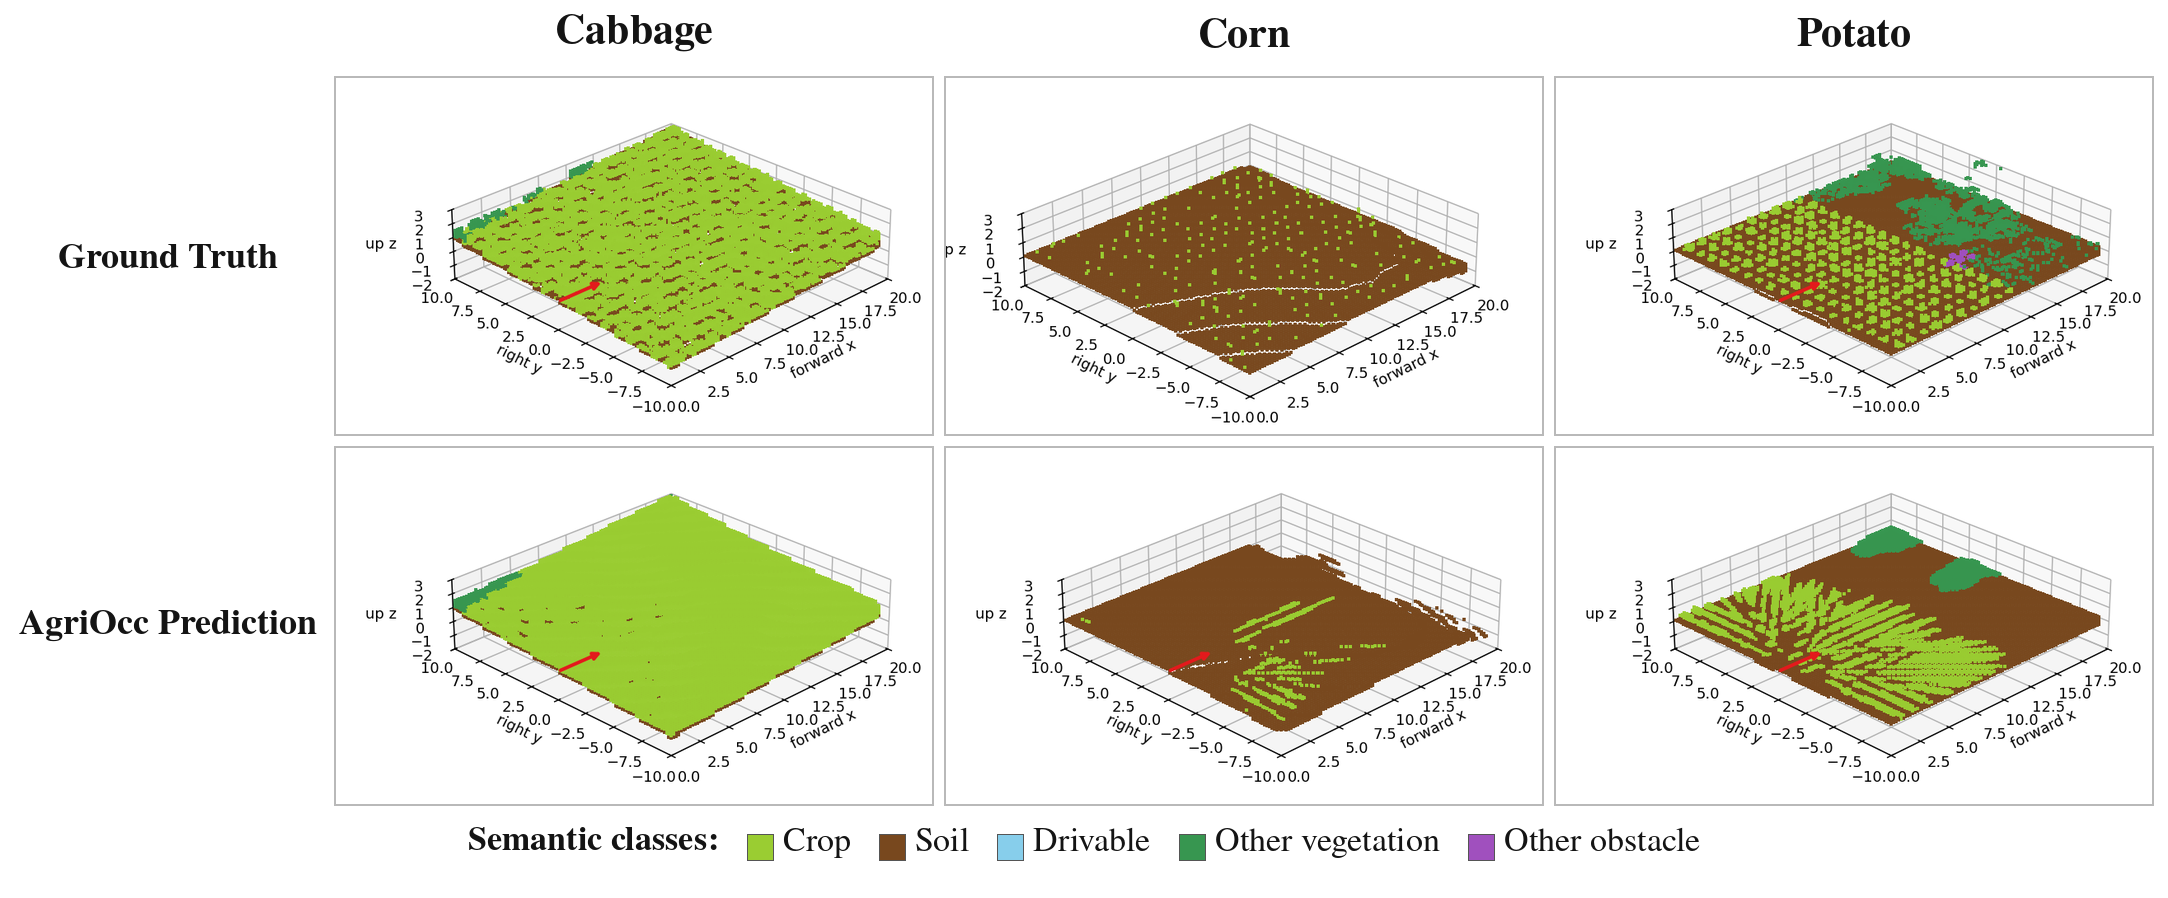
\includegraphics[width=\linewidth]{farmsim_limitations_2x3.png}
\caption{AgriOcc-Dataset 上的局限性示例。第一行为真值标签，第二行为对应的 AgriOcc 预测；三列从左至右分别为卷心菜、玉米和马铃薯场景。密集作物的株间间隙易被预测为连通区域，而苗期等小尺度作物容易出现漏检或范围不足。}
\label{fig:limitations}
\end{figure}

\section{结论与展望}\label{sec:conclusion}

本文提出 AgriOcc，用三路前视图像直接预测农业机器人坐标系下的前方当前三维语义占用。
该框架以GeoVis-BEV 编码器和 Agri-AMoE 三维占用解码器为核心。
GeoVis-BEV 编码器以 GVAD 从可靠可见区域构造锚点上下文，并保持局部可变形采样；
同时以近远场查询布局将编码预算优先分配给近场精细结构。
Agri-AMoE 则将最终 BEV 表征提升为由梯度能量自适应路由的三维混合专家特征体。
在 AgriOcc-Dataset 上，AgriOcc 以 55.74M 参数取得 56.99\% mIoU；
ORAD-3D 迁移结果进一步表明，AgriOcc-Dataset 预训练能够为真实野外和农田空间提供有效的三维占用初始化。

AgriOcc 将农业环境中的作物、地面、自由空间和障碍物统一编码为可直接供规划使用的三维语义接口。
GeoVis-BEV 编码器提供面向农业前向视野的几何感知表征，
Agri-AMoE 则将该表征转化为适配多类空间结构的三维占用特征。
该研究范式可进一步服务于动态作业场景建模、株间细缝与植株结构的精细表达，
以及以语义占用为中间状态的通行性预测、避障和闭环规划。

未来将进一步面向真实农田的光照、天气、作物生长期与传感器扰动构建更丰富的跨域训练策略；
引入选择性激活的高分辨率近场查询，以提升株级作物间隙和细粒度边界的表达；
并将 AgriOcc 的占用表征与风险感知通行性分析、轨迹优化和闭环导航深度耦合。
最终，语义占用有望成为连接农业机器人感知、决策与控制的稳定三维基础模型接口。

\section*{数据与代码可得性}
AgriOcc-Dataset 的构建流程、类别定义与标注生成方式见第\ref{sec:dataset_construction}节。
本研究所用数据集与代码计划在论文接收后公开发布，供非商业研究使用。


\section*{利益冲突声明}
作者声明不存在可能影响本文研究工作的利益冲突。

\bibliographystyle{cas-model2-names}
\bibliography{references}
\end{document}
